\section{Case Study Results} \label{sec:casestudyresults}
In this section, we evaluate our approaches by answering two research questions.

\subsection*{RQ1: How well can we model system performance under varying workloads?}

\subsubsection*{Motivation}
In order to use black-box machine learning models to detect performance regressions under varying workloads, we first need to understand whether such black-box models could accurately model the performance of a software system under varying workloads.
Although prior research demonstrates promising results of using black-box models to capture the relationship between system performance and logs~\citep{Yao:2018:LSL:3184407.3184416,DBLP:conf/issre/FarshchiSWG15},
these models are built on predefined in-house workloads instead of varying field workloads. 
If such black-box models are sensitive to the variance in the workloads, they may not be suitable for modeling the performance of software systems under the field workloads from real end users.

\subsubsection*{Approach}
In order to understand the black-box models' ability for modeling system performance under varying workloads, we train the models on one set of workloads and evaluate the performance of the models on a different set of workloads (i.e., \emph{unseen} workloads).

\noindent\textbf{Modeling for the open source systems. }
For each open source system (i.e., OpenMRS and Apache James), we select the version of the system that is without performance regressions. We first run the system with four different concurrent workloads (i.e., \emph{4W}) and collect the logs and performance metrics. In order to ensure having new workloads to the system, we conduct another run by having an additional concurrent workload, i.e., having five different concurrent workloads (i.e., \emph{5W}). We build the performance models using the data that is generated by running the \emph{4W} workloads and apply the model on the data that is generated by running the \emph{5W} workloads. 
We evaluate the prediction performance of the black-box models on the 5W workloads by comparing the predicted performance and the measured performance.

\noindent\textbf{Modeling for the industry system. }
For System X, we directly use the field data that is generated by workloads from the real end users. For each release cycle with $n$ days, we use the data from the first $n/2$ days to build the models and apply them on the data from the second $n/2$ days to evaluate the prediction performance of the models. We would like to note that there exists no control on the end users for applying any particular workload, and that all the data is directly retrieved from the field with no interference on the behavior of the end users. 

\noindent\textbf{Analysis of modeling results. }
We calculate the prediction errors of the models on the new workloads (i.e., the \emph{5W} workloads for the open source systems and the second $n/2$-day workloads for System X).
In order to understand the magnitude of the prediction errors, we use the prediction errors of the models on the old workloads (i.e., the $4W$ workloads for the open source systems and the first $n/2$-day workloads for System X) as baselines. The baseline prediction errors are calculated using a 10-fold cross validation to avoid the bias of having the same training and testing data.  
\begin{itemize}
    \item \textbf{Median relative error}. The difference between the predicted performance and the measured performance, normalized by the measured performance.
    \item \textbf{p-value} (Mann-Whitney U). In order to understand whether the models trained on the old workloads can equivalently capture the system performance under the new workloads, we use the Mann-Whitney U test~\citep{nachar2008mann} to determine whether there exists a statistically significant difference (i.e., p-value $<$ 0.05) between the prediction errors on the new workloads and the prediction errors on the old workloads. 
    \item \textbf{Effect size} (Cliff\textquotesingle s delta). Reporting only the statistical significance may lead to erroneous results (i.e., if the sample size is very large, the p-value can be very small even if the difference is trivial)~\citep{sullivan2012using}. Therefore, we apply Cliff\textquotesingle s Delta~\citep{cliff1996ordinal} to quantify the effect size of the difference between the prediction errors on the old workloads and the prediction errors on the new workloads. 
\end{itemize}

\subsubsection*{Results}
Table \ref{tab:model_error} shows the detailed results of using six machine learning techniques to model the performance of the studied open source systems (i.e., \emph{OpenMRS} and \emph{Apache James}) under varying workloads.
 The column ``MRE'' shows the  median relative errors of applying the models (trained on the \emph{4W} workloads) on the \emph{4W} workloads and the \emph{5W} workloads, respectively. 
  The columns ``p-value'' and ``effect size'' show the statistical significance and the effect size of the difference between the prediction errors of the models on the \emph{4W} workloads and the prediction errors of the models on the \emph{5W} workloads, respectively. The ``violin plot'' column shows the distribution of the relative prediction errors under the \emph{4W} and \emph{5W} workloads.

\begin{landscape}

\begin{table*}[htbp]
  \centering
  \footnotesize
  \caption{Prediction error details for OpenMRS and Apache James under different workloads. 
 }
    
    \resizebox{.66\paperheight}{!}{
    \begin{tabular}{|c|c|c|c|c|c|c|c|c|c|c|}
    \hline
    \multirow{2}[4]{*}{Model} & \multicolumn{5}{c|}{OpenMRS}          & \multicolumn{5}{c|}{Apache James} \\
\cline{2-11}          & \multicolumn{2}{c|}{MRE} & P-value & Effect size & Violin plot & \multicolumn{2}{c|}{MRE} & P-value & Effect size & Violin plot \\
    \hline
    \multicolumn{1}{|c|}{\multirow{2}[9]{*}{Linear 
Regression}} & \multirow{1}[5]{*}{4W}    & \multirow{1}[5]{*}{3.12\%} & \multirow{2}[9]{*}{\textless 0.01} & \multirow{1}[10]{*}{-0.08} & \multirow{2}[4]{*}{ {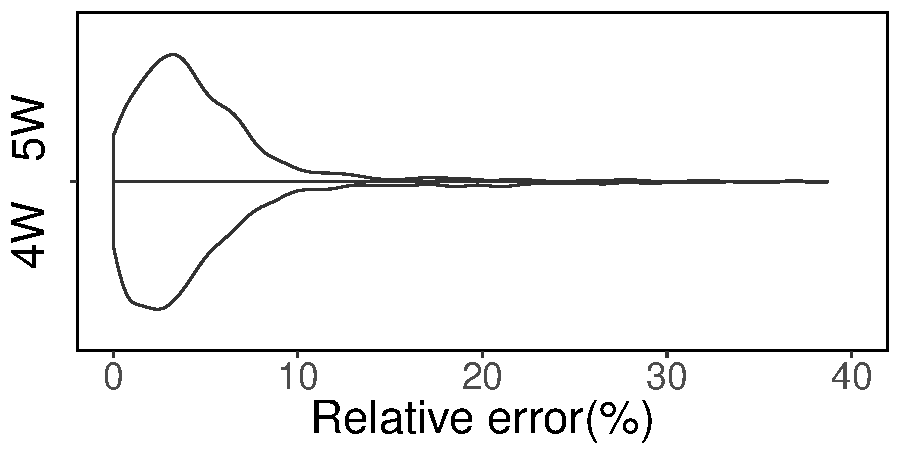
\includegraphics[height=15mm,width=30mm]{openmrs_linear_regression.pdf}}} & \multirow{1}[5]{*}{4W}    & \multirow{1}[5]{*}{23.24\%} & \multirow{2}[9]{*}{0.41} & \multicolumn{1}{c|}{\multirow{2}[9]{*}{N/A}} & \multirow{2}[4]{*}{{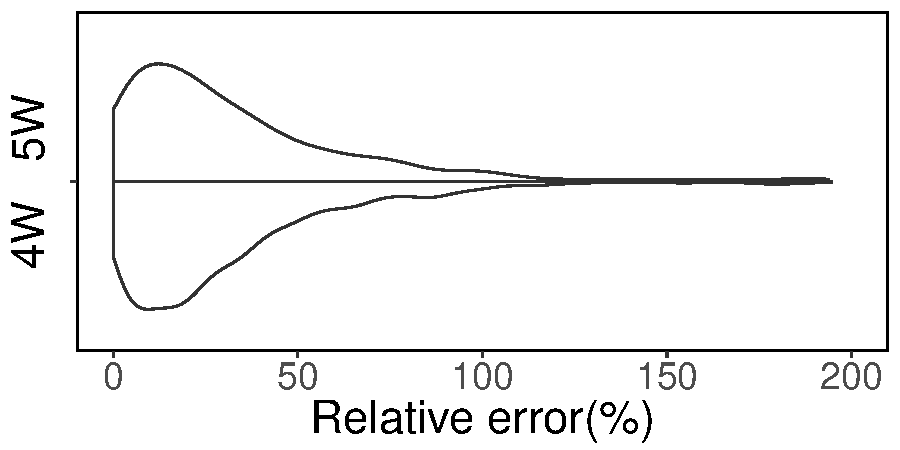
\includegraphics[height=15mm,width=30mm]{jms_linear_regression.pdf}}} \\[4.5mm]
\cline{2-3}\cline{7-8}          & \multirow{1}[5]{*}{5W}    & \multirow{1}[5]{*}{3.58\%} &       & (negligible) &       & \multirow{1}[5]{*}{5W}    & \multirow{1}[5]{*}{23.76\%} &       &       &  \\[4.5mm]
    \hline
    \multicolumn{1}{|c|}{\multirow{2}[9]{*}{Random 
Forest}} & \multirow{1}[5]{*}{4W}    & \multirow{1}[5]{*}{2.36\%} & \multirow{2}[9]{*}{\textless 0.01} & \multirow{1}[10]{*}{-0.09} & \multirow{2}[4]{*}{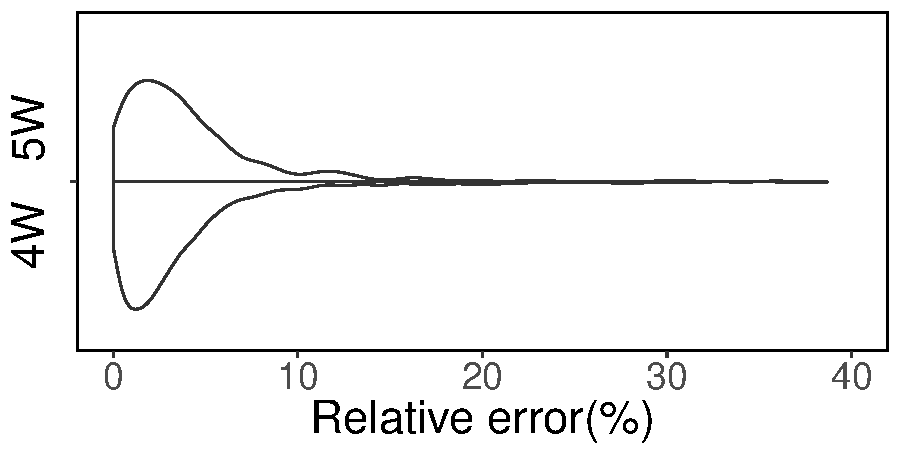
\includegraphics[height=15mm,width=30mm]{openmrs_random_forest.pdf}} & \multirow{1}[5]{*}{4W}    & \multirow{1}[5]{*}{22.99\%} & \multirow{2}[9]{*}{0.42} & \multicolumn{1}{c|}{\multirow{2}[9]{*}{N/A}} & \multirow{2}[4]{*}{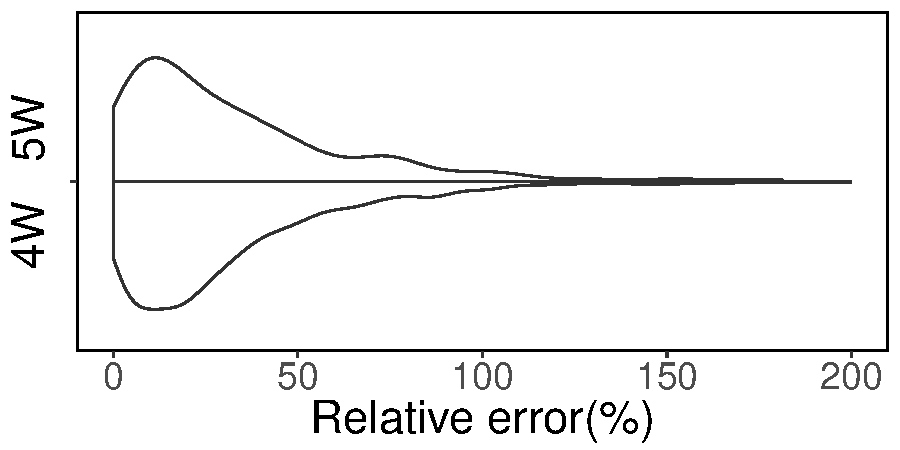
\includegraphics[height=15mm,width=30mm]{jms_random_forest.pdf}} \\[4.5mm]
\cline{2-3}\cline{7-8}          & \multirow{1}[5]{*}{5W}    & \multirow{1}[5]{*}{2.90\%} &       & (negligible) &       & \multirow{1}[5]{*}{5W}    & \multirow{1}[5]{*}{23.08\%} &       &       &  \\[4.5mm]
    \hline
    \multirow{2}[9]{*}{XGBoost} & \multirow{1}[5]{*}{4W}    & \multirow{1}[5]{*}{2.16\%} & \multirow{2}[9]{*}{0.14} & \multirow{2}[9]{*}{N/A} & \multirow{2}[4]{*}{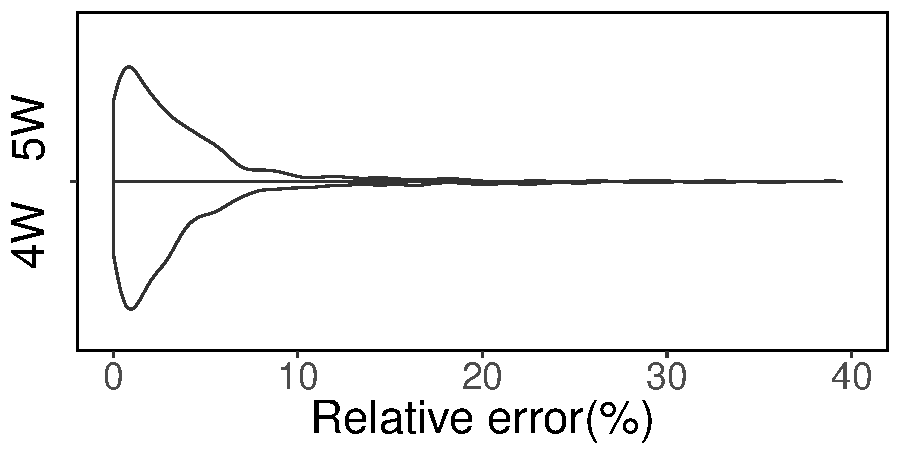
\includegraphics[height=15mm,width=30mm]{openmrs_xgboost.pdf}} & \multirow{1}[5]{*}{4W}    & \multirow{1}[5]{*}{24.29\%} & \multirow{2}[9]{*}{0.44} & \multirow{2}[9]{*}{N/A} & \multirow{2}[4]{*}{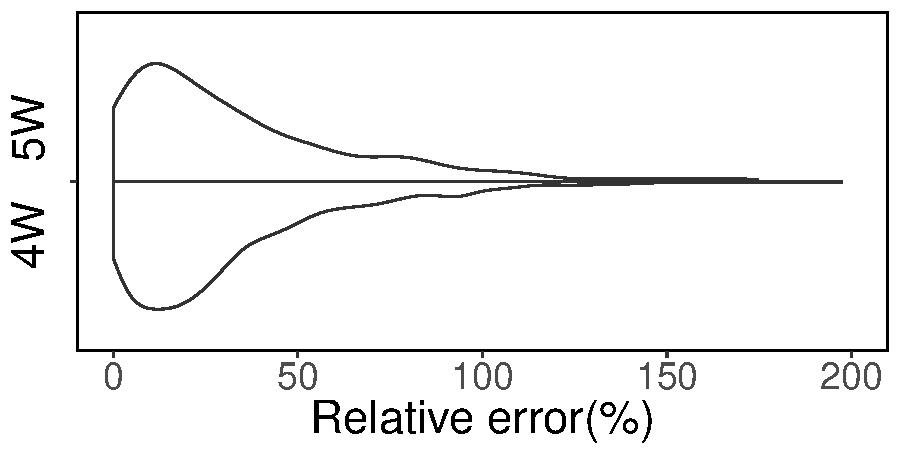
\includegraphics[height=15mm,width=30mm]{jms_xgboost.pdf}} \\[4.5mm]
\cline{2-3}\cline{7-8}          & \multirow{1}[5]{*}{5W}    & \multirow{1}[5]{*}{2.11\%} &       &       &       & \multirow{1}[5]{*}{5W}    & \multirow{1}[5]{*}{24.42\%} &       &       &  \\[4.5mm]
    \hline
    \multirow{2}[9]{*}{CNN} & \multirow{1}[5]{*}{4W}    & \multirow{1}[5]{*}{9.56\%} & \multirow{2}[9]{*}{\textless 0.01} & \multirow{1}[10]{*}{0.12} & \multirow{2}[4]{*}{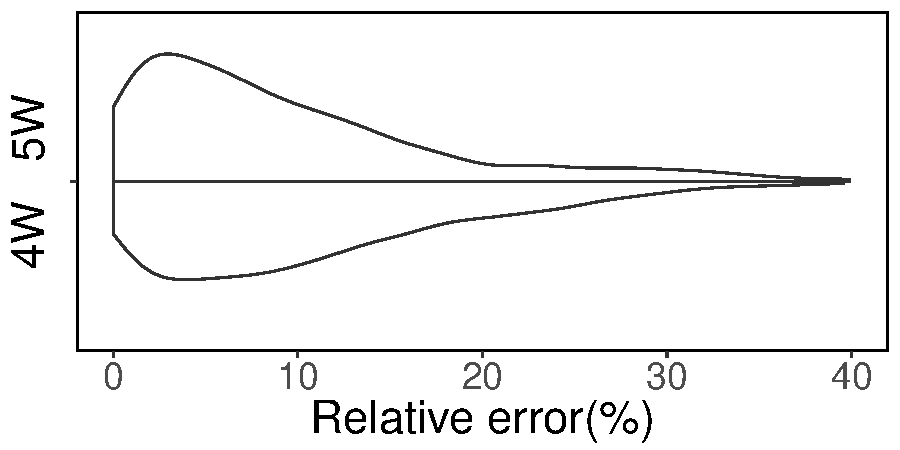
\includegraphics[height=15mm,width=30mm]{openmrs_cnn.pdf}} & \multirow{1}[5]{*}{4W}    & \multirow{1}[5]{*}{33.61\%} & \multirow{2}[9]{*}{0.11} & \multicolumn{1}{c|}{\multirow{2}[9]{*}{N/A}} & \multirow{2}[4]{*}{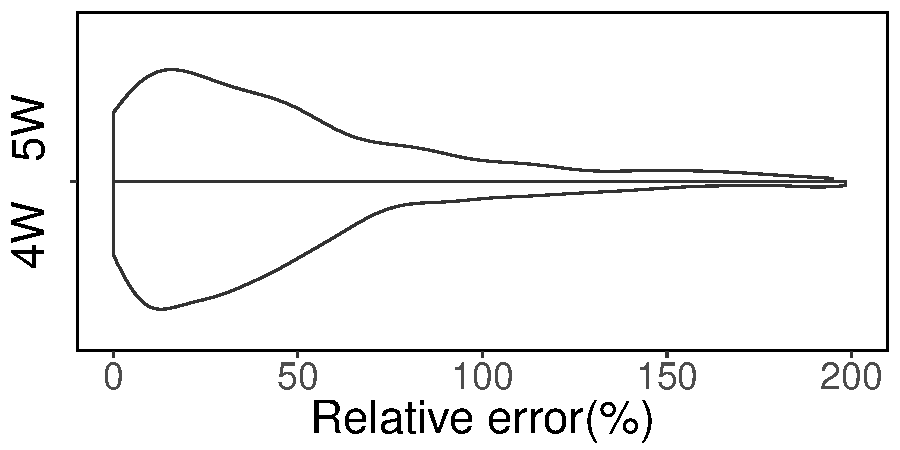
\includegraphics[height=15mm,width=30mm]{jms_cnn.pdf}} \\[4.5mm]
\cline{2-3}\cline{7-8}          & \multirow{1}[5]{*}{5W}    & \multirow{1}[5]{*}{7.47\%} &       & (negligible) &       & \multirow{1}[5]{*}{5W}    & \multirow{1}[5]{*}{37.51\%} &       &       &  \\[4.5mm]
    \hline
    \multirow{2}[9]{*}{RNN} & \multirow{1}[5]{*}{4W}    & \multirow{1}[5]{*}{5.63\%} & \multirow{2}[9]{*}{0.32} & \multirow{2}[9]{*}{N/A} & \multirow{2}[4]{*}{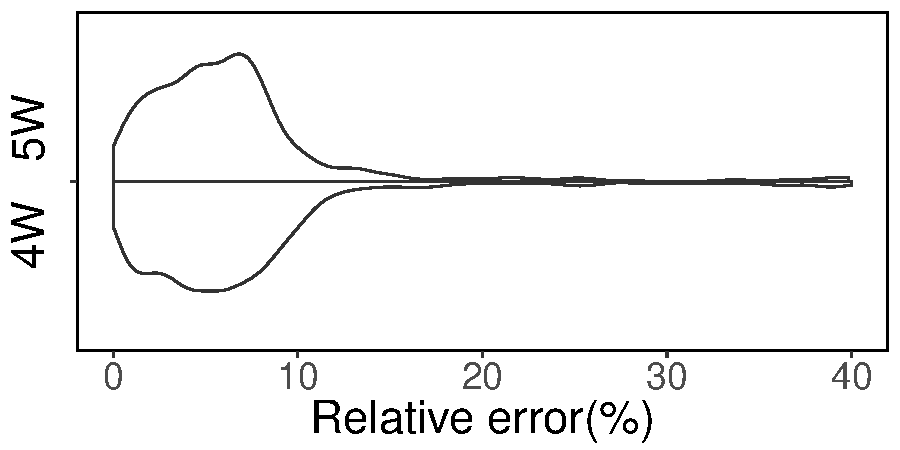
\includegraphics[height=15mm,width=30mm]{openmrs_rnn.pdf}} & \multirow{1}[5]{*}{4W}    & \multirow{1}[5]{*}{51.34\%} & \multirow{2}[9]{*}{0.01} & \multirow{1}[10]{*}{0.07} & \multirow{2}[4]{*}{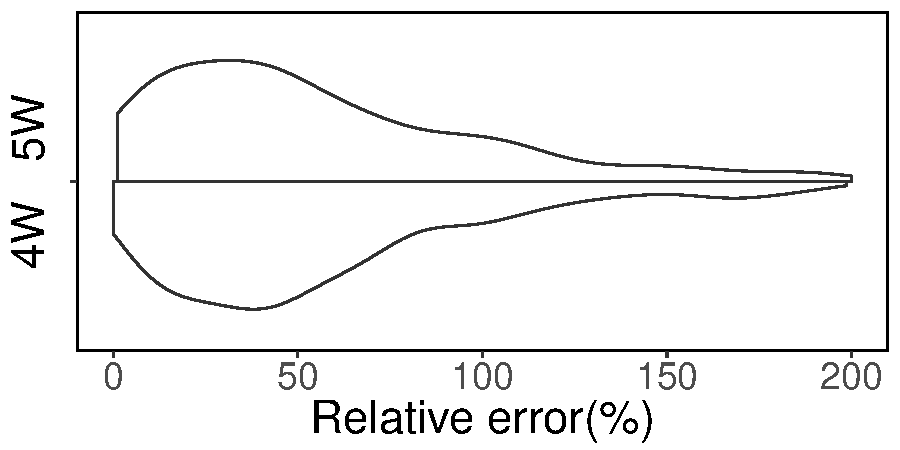
\includegraphics[height=15mm,width=30mm]{jms_rnn.pdf}} \\[4.5mm]
\cline{2-3}\cline{7-8}          & \multirow{1}[5]{*}{5W}    & \multirow{1}[5]{*}{5.73\%} &       &       &       & \multirow{1}[5]{*}{5W}    & \multirow{1}[5]{*}{47.22\%} &       & (negligible) &  \\[4.5mm]
    \hline
    \multirow{2}[9]{*}{LSTM} & \multirow{1}[5]{*}{4W}    &\multirow{1}[5]{*}{ 4.53\%} & \multirow{2}[9]{*}{\textless 0.01} & \multirow{1}[10]{*}{-0.25} & \multirow{2}[4]{*}{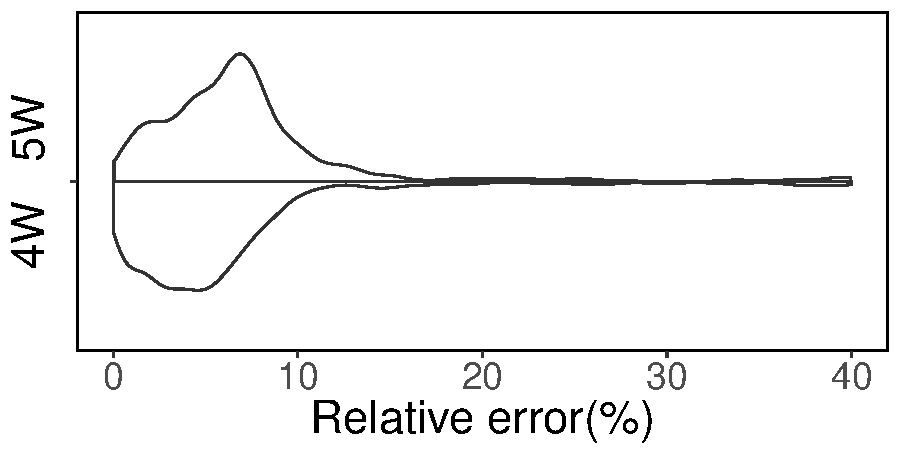
\includegraphics[height=15mm,width=30mm]{openmrs_lstm.pdf}} & \multirow{1}[5]{*}{4W}    & \multirow{1}[5]{*}{34.88\%} & \multirow{2}[9]{*}{\textless 0.01} & \multirow{1}[10]{*}{-0.27} & \multirow{2}[4]{*}{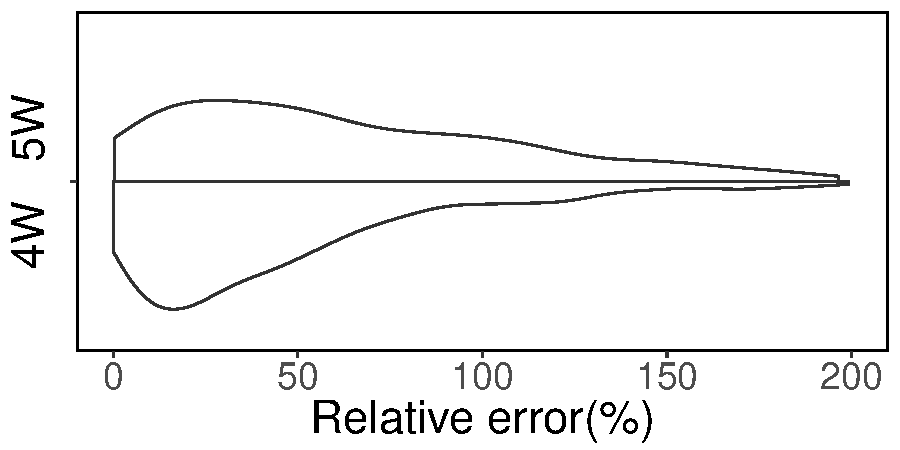
\includegraphics[height=15mm,width=30mm]{jms_lstm.pdf}} \\[4.5mm]
\cline{2-3}\cline{7-8}          & \multirow{1}[5]{*}{5W}    & \multirow{1}[5]{*}{6.42\%} &       & (small) &       & \multirow{1}[5]{*}{5W}    & \multirow{1}[5]{*}{57.11\%} &       & (small) &  \\[4.5mm]
    \hline
    \end{tabular}}
    Note: The column ``MRE'' presents the median relative errors.\hfill
  \label{tab:model_error}%
\end{table*}%
\end{landscape}

\noindent\textbf{Our black-box models can accurately model the performance of the studied systems using the dynamic runtime activities that are recorded in the logs.} 
As shown in Table \ref{tab:model_error}, the XGBoost model achieves the best results for modeling the performance of the OpenMRS system, with a median relative error of 2.11\% on the \emph{5W} workloads (i.e., the new workloads) and a median relative error of 2.16\% on the \emph{4W} workloads (i.e., the baseline workload). 
The random forest model achieves the best results for Apache James, reaching a median relative error of 22.99\% and 23.08\% for the \emph{4W} workloads and \emph{5W} workloads, respectively. 
All the machine learning models achieve better results for the OpenMRS system than the results for the Apache James system.
The less-promising results for the Apache James system might be explained by the latency between the actual activities of the mail server system and the recorded logs. For example, the system can take an extended period of time to process an email with a large attachment, while a log about the successful processing of the email is only printed after the processing period.

\noindent\textbf{The traditional models (e.g., linear regression and random forest) outperform the deep neural networks (e.g., CNN and RNN) for modeling the performance of the studied systems.}
As shown in Table~\ref{tab:model_error}, for both the OpenMRS and the Apache James systems, the three traditional models achieve better results than the three deep neural networks for modeling the system performance.
These results indicate that the relationship between the system performance and the runtime activities recorded in the logs can be effectively captured by the simple traditional models.
Such results also agree with a recent study~\citep{DacremaArxiv2019} that compares deep neural networks and traditional models for the application of automated recommendations.


\noindent\textbf{Our black-box models can equivalently explain the performance of a system under new workloads that are unseen when constructing the models.}
Table~\ref{tab:model_error} shows the statistical significance (i.e. the p-value) and the effect size of the difference between the prediction errors of applying the old models (i.e., trained from the \emph{4W} workloads) on the new workloads (i.e., the \emph{5W} workloads) and applying the old models on the old workloads (i.e., the \emph{4W} workloads). 
Table \ref{tab:model_error} also compares the distributions of the prediction errors for the \emph{4W} and \emph{5W} workloads.
The prediction errors of most of the models (except LSTM) have either statistically insignificant or negligible difference between the \emph{4W} and the \emph{5W} workloads, indicating that the models trained from the old workloads can equivalently model the system performance under new workloads.
The LSTM model results in a \emph{small} difference of the predictions errors between the \emph{4W} and the \emph{5W} workloads. We suspect that the complex LSTM model is likely over-fit towards the training workloads.

Due to an NDA, the detailed results of using the machine learning techniques to model the performance of the industry system (i.e, System X) are not presented in this paper. However, the results are similar to the shown results for the open source systems. In particular, when modeling the performance of all 10 studied versions of System X, the prediction errors are all between 10\% to 20\%. In addition, when we evaluate the models with different workloads, the differences between prediction errors are all either statistically insignificant or with negligible/small effect sizes.



\hypobox{Simple traditional models (e.g., linear regression and random forest) can accurately capture the relationship between the performance of a system and its dynamic activities that are recorded in logs, with varying workloads.
}

\subsection*{RQ2: Can our approach detect performance regressions under varying workloads?}

\subsubsection*{Motivation}

In traditional performance testing, in order to detect performance regressions, performance analysts compare the performance data of two versions of a software system that is generated by running the same workloads from the same performance test suites. 
However, in a field environment, as the workloads of the systems are constantly changing, it is almost impossible to run two software versions on the same workloads to detect performance regressions.
The results of RQ1 show that our black-box models can accurately capture the performance of a software system even under new workloads that are unseen when training the models.
Therefore, in this research question, we would like to leverage such black-box models to detect performance regressions when the workloads of the two versions of a system are not consistent.

Running the systems for hours or days before discovering performance regressions incurs a high cost. As the systems are already running in the field, any delay in detecting the performance regressions may pose huge impact on the end users. Hence, a desired approach in practice should be able to detect performance regression in a timely manner. Therefore, we also want to study how fast our approaches can detect performance regressions. 

\subsubsection*{Approach}

The results from RQ1 show that random forest and XGBoost have the lowest prediction errors when modeling performance (cf. Table~\ref{tab:model_error}). Since XGBoost requires resource-heavy fine-tuning, we opt to use random forest in this research question. For the open source systems, we first build the performance models from running the systems without performance regressions under the \emph{4W} workloads (i.e., a combination of four different concurrent workloads). We then run the systems without performance regressions under the \emph{5W} workloads (i.e., a combination of five different concurrent workloads). Ideally, our approach should not detect performance regressions from these runs. 
We use such results as a baseline to evaluate the effectiveness of our approach for detecting performance regressions under the new workloads (i.e., the \emph{5W} workloads). 
Afterwards, we run the systems with the performance regressions (cf. Table~\ref{tab:workloaddeisign}) under the \emph{5W} workloads. Our approach should be able to detect performance regressions from these runs.

For the System X from the industry, for every new release, we use our approach to compare the field data from the new release and the previous release to determine whether there are performance regressions. Since there are no injected or pre-known performance regressions, we present the detected performance deviance to the developers of the systems and manually study the code changes to understand whether the detection results are correct. For the releases that are detected as not having performance regressions, we cannot guarantee that these releases are free of performance regressions. However, we also present the results to the developers to confirm whether there exist any users who report performance-related issues for these releases. If so, our detection results may be considered false.

Finally, to study how fast our approaches can detect performance regressions, for the new versions of the systems that have performance regressions, we only use the first 15-minute data and apply our approach to detect the performance regressions. Then, we follow an iterative approach to add another 5-minute data to the existing data, until our approach can detect the performance regressions (i.e., with a medium or large effect size that is higher than the baseline). 

\subsubsection*{Results}

\noindent\textbf{Our black-box-based approaches can effectively detect performance regressions under varying workloads.}
Table~\ref{tab:predictionresult_rq2} shows the results of our three approaches of performance regression detection (cf. Section~\ref{sec:comparions-approaches}) on OpenMRS and Apache James. We find that with all three approaches, when there are known performance regressions between two versions, the statistical analysis always shows significant difference between the two versions with medium or large effect sizes. In addition, the effects sizes from Approach 1 and 2 are negative, confirming the existence of performance regressions (negative values indicate performance regression and positive values indicate performance improvement). 

When we compare the effect sizes with the baseline, i.e., running our approaches with systems without performance regressions but under two different workloads, we find that the baseline effect sizes are always smaller than the corresponding ones with performance regressions, except when detecting the regression in v3 of OpenMRS. We consider the reason being the nature of the regression in v3, i.e., an injected delay. Since our considered performance metric is the CPU usage and such a delay may not have large impact on the CPU usage, it is difficult for our approaches to detect such a regression. 


\begin{table}[tbh]
  \centering
  \tiny
  \tabcolsep=0.14cm
  \caption{Performance regression detection results for OpenMRS and Apache James. }
    \begin{tabular}{|c|c|c|c|c|c|c|c|}
    \hline
    \multicolumn{8}{|c|}{OpenMRS} \\
    \hline
    \multicolumn{2}{|c|}{Versions} & \multicolumn{2}{c|}{Approach 1} & \multicolumn{2}{c|}{Approach 2} & \multicolumn{2}{c|}{Approach 3} \\
    \hline
    \multicolumn{1}{|p{0.7cm}<{\centering}|}{Old\newline{}version} & \multicolumn{1}{|p{0.7cm}<{\centering}|}{New\newline{}version} & \multirow{1}[3]{*}{P-value} & \multirow{1}[3]{*}{Effect size} & \multirow{1}[3]{*}{P-value} & \multirow{1}[3]{*}{Effect size} & \multirow{1}[3]{*}{P-value} & \multirow{1}[3]{*}{Effect size} \\
    \hline
    v0 & v0 & $\ll$0.001 & 0.39 (medium) &  $\ll$0.001 & 0.36 (medium) & $\ll$0.001 & 0.17(small) \\
    \hline
    v0 & v1 & $\ll$0.001 & -0.59 (large) & $\ll$0.001 & -0.69 (large) & $\ll$0.001 & 0.38 (medium) \\
    \hline
    v0 & v2 & $\ll$0.001 & -0.44 (medium) & $\ll$0.001 & -0.63 (large) & $\ll$0.001 & 0.37 (medium) \\
    \hline
    v0 & v3 & $\ll$0.001 & -0.36 (medium) & $\ll$0.001 & -0.42 (medium) & $\ll$0.001 & 0.53 (large) \\
    \hline
    v0 & v4 & $\ll$0.001 & -0.69 (large) & $\ll$0.001 & -0.76 (large) & $\ll$0.001 & 0.51 (large) \\
    \hline
    \hline
    \multicolumn{8}{|c|}{Apache James} \\
    \hline
    \multicolumn{2}{|c|}{Versions} & \multicolumn{2}{c|}{Approach 1} & \multicolumn{2}{c|}{Approach 2} & \multicolumn{2}{c|}{Approach 3} \\
    \hline
    \multicolumn{1}{|p{0.7cm}<{\centering}|}{Old \newline{}version} & \multicolumn{1}{|p{0.7cm}<{\centering}|}{New \newline{}version} & \multirow{1}[3]{*}{P-value} & \multirow{1}[3]{*}{Effect size} & \multirow{1}[3]{*}{P-value} & \multirow{1}[3]{*}{Effect size} & \multirow{1}[3]{*}{P-value} & \multirow{1}[3]{*}{Effect size} \\
    \hline
    3.0m2 & 3.0m2 & 0.008 & 0.09 (negligible) & $\ll$0.001 & -0.12 (negligible) & $\ll$0.001 & -0.03 (negligible) \\
    \hline
    3.0m2 & 3.0m1 & $\ll$0.001 & -0.65 (large) & $\ll$0.001 & -0.76 (large) & $\ll$0.001 & 0.41 (medium) \\
    \hline
    3.0m2 & 2.3.2 & $\ll$0.001 & -0.90 (large) &$\ll$0.001 & -0.93 (large) & $\ll$0.001 & 0.82 (large) \\
    \hline
    \end{tabular}\\
    Note: For all the old versions, we use four concurrent workloads and for all the new versions with and without regressions, we use five concurrent workloads (one extra workload).\hfill
  \label{tab:predictionresult_rq2}%
\end{table}%

For all the 10 releases of System X, our approaches detected performance regressions from one release.
All three approaches detected performance regressions from the release with large effect sizes when compared with the previous release.
All three approaches did not detect performance regressions from the other nine releases (i.e., with either statistically insignificant difference or negligible effect sizes when compared with the previous release). 
By further investigating the release with performance regressions, we observed that developers added a synchronized operation to lock the resources that are responsible for generating a report, in order to protect the shared resources under the multi-thread situation. However, the reporting process is rather resource-heavy, resulting in significant overhead for each thread to wait and acquire the resources. Thus, the newly added lock causes the performance regression. After we discussed with the developers who are responsible for this module, we confirmed that this synchronized operation introduced performance regression to the software. 
In addition, for all the nine releases from which our approaches did not detect performance regressions, the developers of System X have not yet received any reported performance issues from the end users till the day of writing this paper.


\noindent\textbf{Comparing the prediction errors is more effective than comparing the prediction values when detecting performance regressions between two versions.}
We observe that for OpenMRS, the differences between the prediction values using Approach 1 and 2 can still be medium (0.39 and 0.36) even for the baseline (i.e., without regressions).
On the other hand, when comparing the prediction errors instead of the prediction values, i.e, using Approach 3, the baseline without regressions has only a small effect size (0.17).
Such a smaller baseline effect size makes Approach 3 easier to be adopted in practice, i.e., without the need of spending efforts searching for an optimal threshold on the effect size to detect performance regressions. However, Approach 3 only shows the deviance of the prediction errors without showing the direction of the performance deviance, thus it cannot distinguish a performance regression from a performance improvement. Hence, Approach 3 may be used first to flag the performance deviance then be combined with other approaches in practice to determine whether the performance deviation is a performance regression or a performance improvement.


\noindent\textbf{Our approaches can detect performance regressions as early as 15 minutes after running a new version.}
Table~\ref{tab:howearly} shows the earliest time that our approach can detect performance regressions in the studied open source systems. We find that all the performance regressions in the open source systems can be detected by at least one approach with less than 20-minute data from the new version. In particular, the regressions from both versions of Apache James and three versions of OpenMRS can even be detected using only the first 15-minute data. The ability of early detection eases the adoption of our approaches in the practices of testing in the field, where performance regressions are detected directly based on the field data, instead of using dedicated performance testing. 
 
\begin{table}[tbh]
  \centering
  \caption{The earliest time for our approaches to detect regressions in the two open source systems.}
    \begin{tabular}{c|cccc|cc}
    \hline
          & \multicolumn{4}{c|}{OpenMRS}  & \multicolumn{2}{c}{Apache James} \\
\cline{2-7}          & v1    & v2    & v3    & v4    & 3.0m1 & 2.3.2 \\
    \hline
    Approach 1 & 60 mins & 160 mins & 15 mins & 15 mins & 15 mins & 15 mins \\
    Approach 2 & 20 mins & 50 mins & 15 mins & 15 mins & 15 mins & 15 mins \\
    Approach 3 & 45 mins & 15 mins & 15 mins & 15 mins & 15 mins & 15 mins \\
    \hline
    \end{tabular}%
  \label{tab:howearly}%
\end{table}%



\hypobox{All three approaches can successfully detect performance regression under varying workloads, requiring data from a very short period of time (down to 15 minutes). 
Comparing the prediction errors is more effective than comparing the prediction values for detecting performance regressions between two versions.
}


